\documentclass[a4paper, 10pt]{article}
\usepackage{float}
\usepackage{graphicx}
\usepackage{subcaption}
\usepackage{hyperref}

% Title Page
\title{Skills Development Challenge for India \\ Charity Insights Scheme: Asha for Education}
\author{Vaibhav Krishnakumar \\ \textsc{Imperial College London}}
\date{July 2015}
% End Title Page

\begin{document}

\pagenumbering{gobble}
\maketitle 

\vspace{50pt}

\includegraphics[scale=0.9]{asha_logo.png}
\vspace{30pt}

\includegraphics[scale=0.8]{imperial_logo.jpg}

\newpage
\pagenumbering{arabic}

\section*{Introduction}
\subsection*{Purpose}
This report is the product of a month-long internship with Asha for Education, an Indian charity with over 60 international offices. It provides a summary of key research papers in the fields of youth unemployment and an overview of the skills development challenges that India faces over the next 25 years. It then gives an idea of Asha's involvement in this sector and the work we are doing to change the status quo.

\subsection*{Context}

\noindent There are 1.2 billion people worldwide aged between 15 and 24 years old; 75 million of them are looking for jobs \textsuperscript{[1]}. This demographic dividend is a huge opportunity for growth - equally, if the situation is not handled correctly, they could become a burden on society and governments. Countries such as China have, over the last few decades, taken advantage of this by tailoring policies to tackle the skill shortage in the workforce; they are now the manufacturing powerhouse of the world. India must follow suit and do the same to try and replicate their success. \\

\begin{figure}[H]
	\centering
		\begin{subfigure}[b]{0.75\textwidth}
			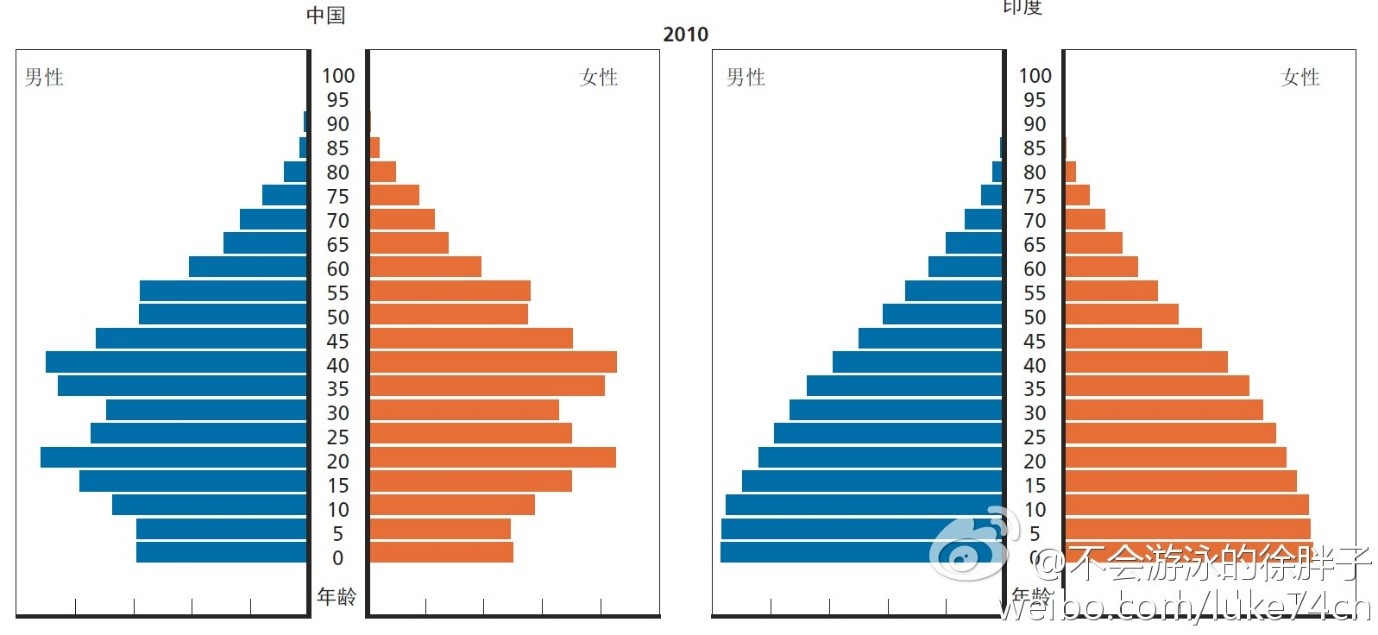
\includegraphics[scale=0.60]{demographics2010.jpg}
			\caption{2010}
		\end{subfigure}
		\begin{subfigure}[b]{0.75\textwidth}		
			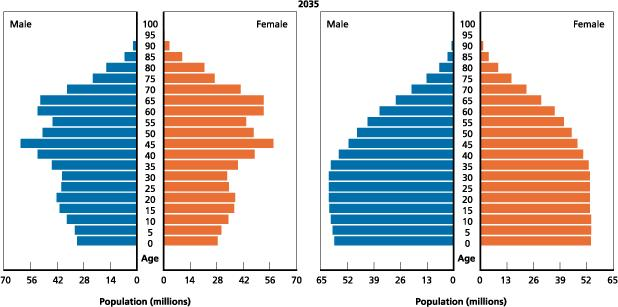
\includegraphics[scale=0.44]{demographics2035.jpg}
			\caption{2035 (projected)}
		\end{subfigure}
	\caption{Population Demographics: China (left), India (right); Male (blue), Female (orange) \textsuperscript{[11]}}
    \label{fig:demographics}
\end{figure}

\noindent Figure~\ref{fig:demographics} illustrates this - the projected population demographics for 2035 shows China's ageing population and India's demographic dividend. The dividend is predicted to last until 2040 \textsuperscript{[5]}; by then, India needs to implement the policies to ensure that the youth are skilled and can face the challenges that a growing economy brings. \\

\noindent Youth unemployment rates tend to be significantly higher than their adult counterparts. This is mainly due to minimal exposure to work, resulting in a lack of soft skills that comes only with experience \textsuperscript{[1][2]}. There is also a knock on effect on employed youth, who are increasingly in lower quality, less well paid jobs. The focus moves towards  earning an income, however meagre, as opposed to improving one's career aspirations \textsuperscript{[1]}. The situation seems bleak but there is ongoing research into various programmes to address this supply-demand mismatch in skills. The aim is to look at some such schemes and judge them based on a standardised system.  

\section*{Current Labour Market in India}
\subsection*{Supply}

\noindent The current labour force in India is about 460 million, of which 431 million are aged between 15 and 59 \textsuperscript{[5]}. Table \ref{sector}, adapted from the NSS Planning Commision's 2010 \textsuperscript{[7]} survey shows the share of workers in different sectors in 2009-10. \\

\begin{table}[H]
\begin{center}
\begin{tabular}{l | c}

Sector & Share (\%) \\ \hline \\
Agriculture & 53 \\ 
Manufacturing & 11 \\
Construction & 11 \\
Trade & 9 \\
Transport & 4 \\
Hospitality and Real Estate & 3 \\
Education & 2 \\
Government & 2 \\
Other & 5 \\

\end{tabular}

\caption{Distribution of workers by sector}
\label{sector}
\end{center}
\end{table}

\noindent A high proportion is based in the agriculture sector and live in rural areas. While farmers have not received formal training, they cannot be considered unskilled in their field of expertise - it is only when they move out of agriculture that this happens. However, low education levels make the transition difficult and results in a skill gap. The effect of this is an illiteracy level of about 30\% \textsuperscript{[5]}  - i.e. approximately 1 in 3 people in the workforce has no basic reading or writing skills. The strategies we discuss can only be effective if built on a basic primary school education which many unfortunately still lack. 

\subsection*{Demand}
The demand in the agricultural sector is perhaps the only one that is met. However, there are still problems to deal with here. Due to limited external input into the system, advances in farming techniques are not taken full advantage of; families pass on acquired skills by word of mouth informally. This raises questions about the sustainability of these farming practises especially with regard to the environmental impact. Equally, the efficiency of farming has to be scrutinised - 80\% of water consumption in India is in agriculture and yet 40\% of the food produced is wasted \textsuperscript{[12]}. \\

\noindent Outside of this sector, finding employment remains a significant challenge. In the second half of the 2000s, there was a net loss of 1 million jobs, with the manufacturing sector taking a big hit \textsuperscript{[5]}. While demand fluctuates by industry, it is clear that more jobs are required as the net change is largely stagnant. Of particular note is that 90\% of India's employment is in the unorganised sector which covers a wide range of jobs usually of lower productivity and income \textsuperscript{[13]}. \\

\begin{figure}[H]
\centering

\begin{subfigure}[b]{0.75\textwidth}
	\begin{tabular}{c | c c c}
	Sector & & Share by Year (\%) & \\
	& 2013 & 2015 & 2020* \\ \hline \\
	Agriculture & 17.4 & 17.0 & 12.0 \\
	Industry & 25.8 & 30.0 & 28.2 \\
	Services & 56.9 & 53.0 & 59.8 \\
	\end{tabular}
	\caption{Recent and Projected(*) values \textsuperscript{[8][9]}}
\end{subfigure}

\begin{subfigure}[b]{0.75\textwidth}
	\centerline{
		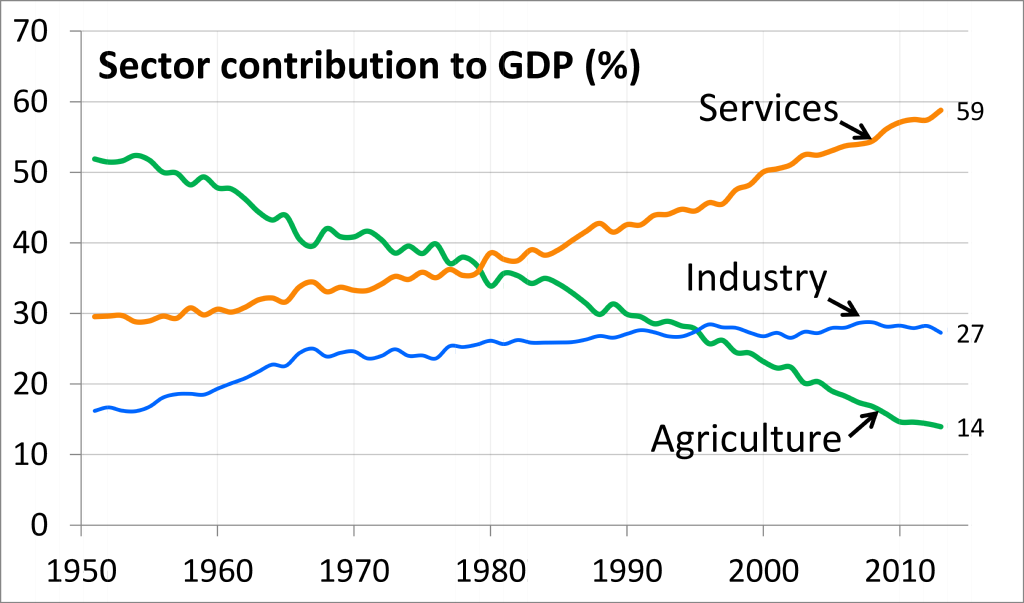
\includegraphics[scale=4]{gdptrend.png}
	}
	\caption{Graph for 60 year trend \textsuperscript{[10]}}
\end{subfigure}
    \label{fig:gdptrend}
	\caption{GDP contribution by sector}
\end{figure}

\section*{Skill Gap in India}
There is a clear mismatch between the skills required by employers and those that prospective employees provide. The key challenge of the skill development programs, whichever is implemented, is to address this inconsistency. Mehrotra's article \textsuperscript{[5]} gives an estimate for the number of people to be 'skilled' by 2020 to counteract the mismatch. Taking into account education levels, sector-specific requirements and making certain assumptions, the number arrived at is 250 million. \\

\noindent As the GDP trends show, there is a transition of labour force from agriculture to industry and services. This exodus, which predicts the share of farming in the labour force to go down to 40\% , results in an increase of untrained workers in the workforce. The paper estimates that only 20\% of the workforce is vocationally trained \textsuperscript{[5]}. If we consider technical training, the numbers are even lower; estimates suggest that a meagre 2.5\% of the workforce has a technical education \textsuperscript{[5]}. \\

\noindent Considering the challenges of a growing economy and the need for skilled labour, these numbers are woefully inadequate. Training 250 million people is a significant burden on the government but one that can lead to huge benefits in the future. Rather than treating this as a challenge, the government should use this as an opportunity for growth. The strategies discussed below can yield the demographic dividend and organisations such as Asha for Education are helping the government implement these strategies. 

\section*{Bridging the Gap}
There are two main strategies we discuss to address the skill gap. They are both common forms of encouraging youth employment. 
\begin{enumerate}
\item Active Labour Market Programs (ALMPs)
\item Technical and Vocational Training and Education (TVETs)
\end{enumerate}

\subsection*{ALMPs}
ALMP is an umbrella term that is used to define all social expenditure (excluding education) which aims to find employment or increase the net income of the beneficiary. Examples include spending on public employment services, market training, schemes that aid school to work transition etc. \textsuperscript{[1]} Four main types of ALMPs are discussed in detail by Kluve et al \textsuperscript{[1]}.

\subparagraph*{1. Training and Development}
Arguably the most widely used, skill training and development is often used in collaboration with other methods to increase employability of an individual as a generic concept. It aims to teach skills such as self-management, teamwork, communication etc., skills which are difficult to pick up for inexperienced youth. It is increasingly important as employers can give job-specific training on recruitment. The skills vary widely in nature and include literacy and numeracy skills, business skills training, training in ICT and are often imparted in internships, placements or entrepreneurial programs. It is often considered as a 'second chance' program in countries, as an alternative to general higher education. \\

\noindent These type of programs are particularly important to bring \textit{additional} youth in employment - not just replace those who are already in employment with better trained employers. A training scheme such as this has to be formalised (e.g. with a certificate) so that it is recognised by employers. It has the advantage of giving the beneficiary transferable skills and doesn't restrict them to a particular vocation. 

\subparagraph*{2. Entrepreneurship}
Particularly in developing countries, formal employment is limited. The common alternative is to set up one's own business but this has many obstacles. The biggest of these is financial - often people do not have disposable income or personal savings to put towards a business. Schemes that promote entrepreneurship can help by providing access to credit, either monetary or in kind, start-up grands or setting up micro-franchising mechanisms. Another setback is the lack of security and credibility in such a venture - the associated risk is off-putting for many youth. Programs could help by providing business advisory services or reduce barriers for entry into a specific market. \\

\noindent Most programs cover the issues comprehensively, often also helping with legal regulations and training. The best (and often only) measure of success is the direct effect on the participant. The business must meet some client needs - it must ideally fill a gap in the current market. Finally, a key idea is sustainability - the business should increase outputs and profits in future years, employing more people so that it has a cyclic effect. An interesting point raised in the paper was the idea to build the training on an existing passion - this can be a powerful motivating factor for the business to succeed from the participant's point of view. 

\subparagraph*{3. Employment Services}
Programs which offer employment services directly tackle the supply-demand mismatch in skills. They work with both unemployed youth and potential employers and are often called "job-matching" schemes. The program deals with participants on a case-by-case basis and is often a service provided by the government - although increasingly, they are subcontracted to private institutions. \\

\noindent For jobseekers, the scheme informs them about the opportunities available and helps build their social capital to create the connections which they lack. This could be through training in 'advertising' (e.g. CV writing, careers guidance, counselling) or networking skills. It can be particularly effective if used with young people who are disconnected from society and who may not want to work at all. The idea is to make searching for a job as painless and efficient as possible. For employers, the converse holds - they are provided information about potential employees and the skills on offer. In addition, this can help reduce some of the cost and risk associated with hiring young or inexperienced people. 

\subparagraph*{4. Employment Subsidies}
The risk associated with first-time workers is a large disincentive to hire them. The government can either provide certain benefits for employers willing to hire first-time workers or act as the employer of last resort. The benefits for the employee are limited - the earnings are low and their skill level does not usually improve. However, it is an increased return on employment and is often targeted at disadvantaged or unskilled workers. The primary aim is to keep them in touch with the labour market and maintain social integration. \\

\noindent There are certain provisions for this to be a successful scheme. The idea is to improve the long term employability of these workers - otherwise, there is excessive dependency on these jobs which prevents a transition to unsubsidised employment. Moreover, there is often stigmatisation against such workers, preventing good integration with the existing workforce. Interestingly, the timing of the program can have an impact on its effectiveness - implementing such a scheme in the agricultural off-season could be beneficial in India. 

\subsection*{TVETs}
TVET programs (or just TVETs) are defined by UNESCO as a collective term for aspects of the educational process (other than general education) which contribute to the study of sciences, technologies and the acquisition of practical skills, aptitudes, understanding and knowledge relating to different sectors in employment. \textsuperscript{[2]} There are 4 key types of TVETs:

\begin{itemize}
\item Technical Education - theoretical preparation focusing on the basic principles of maths and science and their applications. It is usually for occupations that are skilled above craftsmen but below mainstream engineering professions. 
\item Vocational Education - a practical approach to preparation for entry into a designated trade. It usually falls under the jurisdiction of the Department of Education as it is considered part of the formal education system.
\item Vocational Training - preparation for a specific job or occupation with links to the labour market and employment development systems. As a result, it is usually administered by the Department of Labour.
\item Apprenticeship - a combination of on-the-job training with academic and theoretical instructions from an expert in the field. It encourages the "learning-by-doing" approach to jobs
\end{itemize}

\noindent The existing TVET system in India is inadequate and inefficient; before it can be expanded, it must be reformed. \textsuperscript{[3]} This is easier said than done due to financial constraints and the pressure of the demographic dividend. A clear strategy is required before proceeding to make changes. \\

\noindent Currently, less than 3\% of students enrolled in secondary schools undertake a TVET and there is a tendency for students to go into higher education upon completion \textsuperscript{[3]}. TVETs are considered as a second chance at school education rather than a doorway into industry and the workforce \textsuperscript{[4]}. Audience participation is also a good measure for the success of an intervention as the majority are voluntarily run \textsuperscript{[2]}. So a low participation rate suggests that students also do not have faith in the system. Equally, from the employer's point of view, it is more beneficial to hire someone with an education compared to a TVET - any specific skills can be taught on the job as and when required \textsuperscript{[3]}. So TVETs are currently ineffective at making the changes required. \\

\noindent The labour market outcome for TVET graduates has not been very good in recent years. There is limited growth and demand in the manufacturing sector and the relevance of TVETs is questionable as the the skill mismatch is also an issue \textsuperscript{[3]}. The TVETs offered by the ITIs and ITCs (training institutions) does not cater for the informal sector which makes up the majority of India's employment. Apprentices, while common in this sector, continue to be traditional and learnt from an older generation - new technologies are not applied and there is no theoretical grounding. The skills gained are not transferable \textsuperscript{[3]}. \\

\noindent Major reforms are required to ensure that the system can cope with the demands of the next 20 years. The report commissioned by the Government of India \textsuperscript{[3]} suggests changes in 3 key areas:

\subparagraph*{Private Sector}
Increased involvement of the private sector is crucial for the skill mismatch to be addressed. After all, TVET graduates will eventually target this sector for jobs so their input in the intervention will allow them to guide the course to teach the skills required. As they have a vested interest, they may also be willing to fund some of the schemes, at least in part. However, for them to make an impact, they must be involved in running the course and setting the curriculum, not simply in an advisory capacity. The responsibilities must shift in their favour.

\subparagraph*{Government}
Currently, the government is involved heavily with the TVET system. For the reforms to be effective, bureaucratic red tape has to be cut down to the bare minimum. Management of the system is fragmented between various departments at both national and state level; inter-departmental communication is minimal. As a result, institutions have limited vested interest or freedom to improve their performance. A potential change here is for the government to be a supervisor rather than an enforcer - they can setup a national independent authority for TVETs, distribute information on the courses available and standardise the curriculum. However, the imparting of knowledge and skills is best left to each individual state to suit their needs.

\subparagraph*{Funding}
Unit costs in TVETs are typically high, averaging between Rs. 20000 and Rs. 25000 per student per course. However, the majority of expenditure is on staff so critical training input is low. The funding model needs to be made more transparent and future funds should be linked to performance. In particular, the source of funds should be considered - students pay for 5\% of the cost of a course. This is an unreasonably low number, and has potential to increase. At the same time, care must be taken to not shut out students from low income families by having means-tested grants, bursaries etc. There are 3 key beneficiaries from the TVET system - Students, Governments and Employers - so all of them should contribute to the cost of training. \\

\noindent In implementing these changes to the TVET system, India has the distinct advantage of following China's footsteps. China passed the VET Law in 1996 which 	enforced many of the changes discussed; the system was decentralised with local industries involved in setting the curricula \textsuperscript{[14]}. The funding comes primarily from the government (71\%) with companies contributing in training or in the form of taxes \textsuperscript{[14]}. These are changes that India can look to implement in the near future.  

\section*{Asha for Education's Role}
Asha for Education currently has over 70 projects which provide TVET courses to underprivileged youth in India. As a central body organising the funding for these projects, the projects have to be periodically evaluated to ensure they meet the standards required. As a result, a new system will be rolled out; every time a TVET project requests additional funding, they have to answer question which roughly equate to the following indicators.

\subsection*{Indicators}
There are four key indicators while assessing TVETs, as identified by a joint venture involving various international organisations \textsuperscript{[4]}.

\subparagraph*{Finance} 
This deals with two key issues - one is the efficiency of the program in using its available resources. Secondly, this takes into account the economic situation of the region and puts the funding received in context. As a simple example, a TVET project in rural Gujarat is likely to receive less funding than one in central Delhi - irrespective of the quality of these projects. 

\subparagraph*{Access and Participation}
This assesses the equity and inclusion principles of the program. The idea here is that the program has the biggest impact it can for the most amount of people possible. This is measured using the demographic details of the participants by considering their age, gender, socio-economic background, education level etc.

\subparagraph*{Quality}
Arguably the most important metric, this addresses the standards of teaching in addition to the facilities provided. So the training level of teachers, employment statistics of participants after graduation and the availability of equipment and resources is considered under this heading. Of particular importance is the use of ICT in education, something which is essential in the modern world for employment. 

\subparagraph*{Relevance}
This measures the responsiveness of the program to the needs of the labour market. The skills taught by the TVET scheme should match those required by employers. This is best achieved through increased private sector participation as mentioned earlier. However, it is increasingly difficult in a changing labour market such as India's. Of particular importance is the need to fill the skill gap for \textit{new jobs}. 

\subsection*{Metric}
In building the metrics, the indicators are taken into account as general guidelines and more specific questions are formed. The process of finding the questions and the final list are attached in a separate paper written by long-term volunteers with Asha for Education. Responses are taken into account with other details provided (funding to date, regional data, track record of project etc.) to assess how the projects are doing, comparing their aims and outcomes and whether requests for further funding will be approved. 

\section*{References}

The following papers are summarised in the document and were used extensively:

\begin{enumerate}

%1
\item Interventions to Improve Labour Market Outcomes of Youth: A Systematic Review of Active Labour Market Programmes (Kluve et al)

%2
\item Technical and Vocational Education and Training (TVET) Interventions to Improve the Employability and Employment of Young People in Low and Middle-Income Countries: A Systematic Review (Tripney et al)

%3
\item Skill Development in India: The Vocational Education and Training System (The World Bank)

%4
\item Proposed Indicators for Assessing Technical and Vocational Education and Training (IAG-TVET)

%5
\item Estimating India\textsc{\char13}s Skill Gap on a Realistic Basis for 2022 (Mehrotra et al)

%6
\item Conducting influential impact evaluations in China: The experience of the Rural Education Action Project [REAP] (Boswell et al) \\

In addition, the following were used for images or statistics as appropriate: \\

%7
\item NSSO Survey, 2009-10 (\url{http://planningcommission.nic.in/data/datatable/0306/table\%20116.pdf})

%8
\item Central Statistical Office (CSO), 2014 (\url{http://planningcommission.nic.in/data/datatable/0306/table\%203.pdf})

%9
\item World Bank, CSO, DNB; retrieved from \url{http://www.dnb.co.in/India2020economyoutlook/Macro_Economic_Outlook2020.asp}

%10
\item Wikipedia Commons Images, retrieved from  \url{https://commons.wikimedia.org/wiki/File:1951_to_2013_Trend_Chart_of_Sector_Share_of_Total_GDP_for_each_year_India.png}

%11
\item RAND Corporation (\url{http://www.rand.org/pubs/research_briefs/RB9598/index1.html})

%12
\item India Water Portal (\url{http://www.indiawaterportal.org/topics/agriculture})

%13
\item Labour Laws and other Labour Regulations, Planning Commission of India (\url{http://planningcommission.nic.in/aboutus/committee/wrkgrp11/wg11_rplabr.pdf})

%14
\item China's Skill Development System: Lessons for India (Mehrotra et al)

\end{enumerate}

\end{document}